%Conceptuaization diagram
\begin{figure}[ht]
\centering

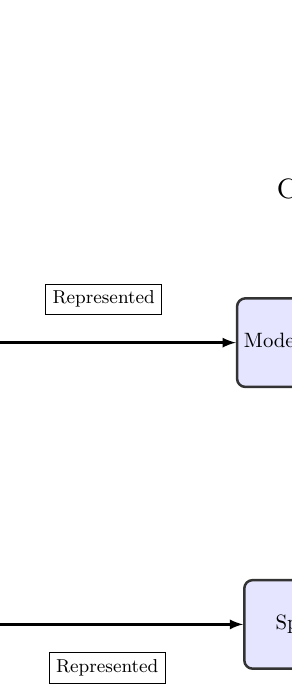
\begin{tikzpicture}[squarednode/.style={rectangle, 
					rounded corners, 
					very thick,
 					minimum width=3cm,
					minimum height=1.5cm,
					draw=black!80, 
					fill=red!10},
					squarednode2/.style={rectangle, 
					rounded corners, 
					very thick,
 					minimum width=3cm,
					minimum height=1.5cm,
					draw=black!80, 
					fill=blue!10}
					]
					
% To reduce all image, transform canvas
% forgets about image size, so 
% we need a bounding box
% This is lame, but works with Eduardo Thesis´s image (now black and white for elegance)

% don´t ask me about theses limits
% I just tried until I found which ones
%workded
\useasboundingbox (3,-4) rectangle (6,4);
\scope[transform canvas={scale=.75}]
         % Your actual drawing


%model nodes
\node[squarednode]  (concept) [anchor = west]{Conceptualization};
\node[squarednode2]  (mlang) [right of = concept, node distance=6cm, anchor=west] {Modeling Language};
\node[squarednode]  (model) [below of = concept, node distance=4cm, anchor=north] {Model};
\node[squarednode2]  (spec) [below of = mlang, node distance=4cm, anchor=north] {Specification};

% Arrows
\path[-latex, double, black, very thick] (concept.south) edge  coordinate[midway](c_to_m) (model.north);

\path[-latex, double, black, very thick] (mlang.south) edge  coordinate[midway](ml_to_s) (spec.north);

\path[-latex, double, black, very thick] (concept.east) edge  coordinate[midway](ml_to_c) (mlang.west);

\path[-latex, double, black, very thick] (model.east) edge  coordinate[midway](m_to_s) (spec.west);


\node [draw] (ml_to_cleg) [above of = ml_to_c, align=center, node distance=1cm, anchor=north]{\small Represented};

\node [draw] (m_to_sleg) [below of = m_to_s, align=center, node distance=1cm, anchor=south]{\small Represented};

\node [draw] (m_to_cleg) [left of = c_to_m, align=center, node distance=0.5cm, anchor=east]{\small Compose};

\node [draw] (ml_to_sleg) [right of = ml_to_s, align=center, node distance=0.5cm, anchor=west]{\small Compose};

\node (abs) [scale = 1.5, above of = concept, align=center, node distance=1.5cm, anchor=south]{\small Abstract};

\node (conc) [scale = 1.5, above of = mlang, align=center, node distance=1.5cm, anchor=south]{\small Concrete};

%\draw [dashed,<-,very thick](designerPathnew.north) |- (designerLegend.east);

    \endscope
\end{tikzpicture}
\caption{Modeling Diagram}
\label{fig:model_diag}
\end{figure}